\documentclass[border=0pt]{standalone}
\usepackage[sfdefault]{roboto}
\usepackage{bm}
\usepackage{makecell}
\usepackage{amsmath}
\usepackage{amssymb}

\usepackage{tikz}

\begin{document}
\begin{tabular}[t]{c|cc}
\multicolumn{3}{l}{
$\bullet\ \ $\textbf{Quantum Annealing} solves quadratic unconstrained binary optimization (\textbf{QUBO}) problems
}\\
\multicolumn{3}{c}{
\textbf{Example Join Ordering:}
}\\
\makecell[tl]{$\bullet\ \ P$: power set of relations to join\\
$\bullet\ \ P_k$: set of elements representing\\\quad joins of $k$ relations, i.e.,\\
\quad $P_k =\{ a|a\in P \wedge |a|=k \} \subseteq P$\\
$\bullet\ \ w_{max}=max(w_i)+c$, where $c>0$\\\quad and $w_i$ represents the cost of join $i$\\
$\bullet\ \ $\textbf{Rewarding joins with lowest costs:}\\
$\quad S_1=\sum_{j=2}^m\sum_{i\in P_j}x_i\cdot (w_i-w_{max})$
}&
\makecell[tc]{
Example\\
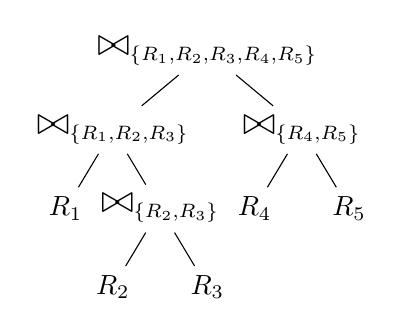
\begin{tikzpicture}
 \node {$\mbox{\Large$\bowtie$}_{\{R_1,R_2,R_3,R_4,R_5\}}$} [sibling distance = 2.4cm, level distance = 1cm]
    child {node {$\mbox{\Large$\bowtie$}_{\{R_1,R_2,R_3\}}$} [sibling distance = 1.2cm]
        child {node {$R_1$}}
        child {node {$\mbox{\Large$\bowtie$}_{\{R_2,R_3\}}$}
            child {node {$R_2$}}
            child {node {$R_3$}}
            }
    } 
    child {node {$\mbox{\Large$\bowtie$}_{\{R_4,R_5\}}$} [sibling distance = 1.2cm]
        child {node {$R_4$}}
        child {node {$R_5$}}
    };
 \end{tikzpicture}}
&
\makecell[tc]{
Constraint:\\
\begin{tikzpicture}
\node {...} [sibling distance = 1.2cm, level distance = 0.7cm]
  child {node {$\mbox{\Large$\bowtie_{z}$}$} 
    child {node {} [sibling distance = 1.2cm]
        child {node{...}
            edge from parent [solid]
        }
        child {node {$\mbox{\Large$\bowtie_{y}$}$}
            child {node{...}
                edge from parent [solid]
            }
            child {node{...}
                edge from parent [solid]
            }
            edge from parent [dotted]
        }
        edge from parent [solid]
    } 
    child {node {...}
        edge from parent [solid]
    }
    edge from parent [dotted]
  };
 \end{tikzpicture}
 \\
 {\Large$y \subseteq z$}
}\\
&
\multicolumn{2}{c}{
\textbf{Punish other combinations:}
}\\&
\multicolumn{2}{c}{
$\Rightarrow S_2=\sum_{i=2}^{m-1}\sum_{j=i}^m \sum_{\substack{y\in P_i\\\wedge z\in P_j\\\wedge y\cap z\neq\emptyset \\\wedge y \nsubseteq z}} x_y*x_z*w_{max}$
}\\
\multicolumn{3}{c}{
\textbf{Minimize $S=S_1+S_2$}
}
\end{tabular}


\end{document}